\entry{Semana del 08/09/2025} 

\section{Lunes 08/09/2025} 
\subsection*{Notas del día:} 
\begin{itemize}
	\item Voy a repetir la calibración con el motor pero llevándome también su posición real desde el software para compara mejor. 
	\item Uso más agua para que esté siempre muy sumergido. Voy a medir además durante más tiempo para llegar bien al estacionario (5 min).  
	
	\item uso 10 Vpp. 
	
	\item Confirmo que cuanto más sumergido está el sensor menos fase hay, o sea, cuando sube el agua y cubre más del alambre la fase se hace negativa, en la calibración hay que multiplicar por ``-". 
	
	\item Frecuencia de 52.676 para más o menos centrar la curva. Está tocando el borde de la tapa el alambre de acero como siempre por la rotación del motor. 
	\item Me parece que voy a aprovechar y llevarme también una escalonada y una rampa sym. 
	\item Todo en 50% de amplitud del motor. 
	\item Antes de la escalonada se cayó un poco de agua. 
	\item Vibra mucho el agua aún con la rampa de 1 minuto. 
	
	\item ¿Soporte estaba electrificado?. 
	
	\item Me llevo rampa escalón del día 2 con 180 s. De la rampa sym del día 1, 8 s de período. 
	\item Tal vez en otro momento probar con seno de distintas frecuencias directamente. 
	
	\item Con la frecuencia de corte en 1000 Hz da muy ruidosa la de max\_1Hz\_10s. Ahora estoy probando con menos porque en el de tiempo real se notaba re bien. Intuyo que tendrá que ver tal vez con la baja amplitud, aunque para la medición del día 1 daba bien incluso con 1000 Hz de corte. por ahí se aflojó algún cable. 
	
	\item Calcular correlación u error relativo después de alinearlas. 
\end{itemize}

Hoy repetí las experiencias de calibración del sensor con el motor lineal moviendo el recipiente con agua destilada, pero teniendo el cuidado de esperar 1 minuto en la medición para que pase el transitorio largo y llevándome además la posición real que reporta el motor usando su software, aunque sin sincronizar ambas mediciones. 

El Montaje fue exactamente el mismo que el del día Miércoles 16/07/2025. Levanté mediciones para el forzado aleatorio con frecuencia máxima de 1 Hz, la rampa simétrica y la escalonada. Usé de nuevo el factor en la amplitud del 50 \%. 



\section{Miércoles 10/09/2025} 
Empecé a armar la charla para la RAFA, para lo cual fue necesario terminar de redondear el análisis a los datos de la calibración. Lo que terminamos haciendo fue: 

\begin{itemize}
	\item Downsamplear la señal del sensor a la misma frecuencia de sampleo que las mediciones de pósición del motor. Para esto simplemente interpolé la señal del sensor (con frecuencia de corte de 100 Hz) y la evalué en los tiempos correspondientes a la $f_s$ del motor. 
	\item Calcular la correlación cruzada entre ambas señales para encontrar la ventana del sensor que mejor coincida con la del motor. 
	\item Graficar una contra la otra y ajustar linealmente para obtener los factores de calibración. 
	\item Calibrar la señal y calcular las diferencias entre ambas. 
	\item Estudiar el histograma y espectro de dichas diferencias.
\end{itemize}

Podemos ver que las ventana de mejor coincidencia entre el motor y el sensor ya cualitativamente da muy bien. 

\begin{figure}[th!]
	\centering
	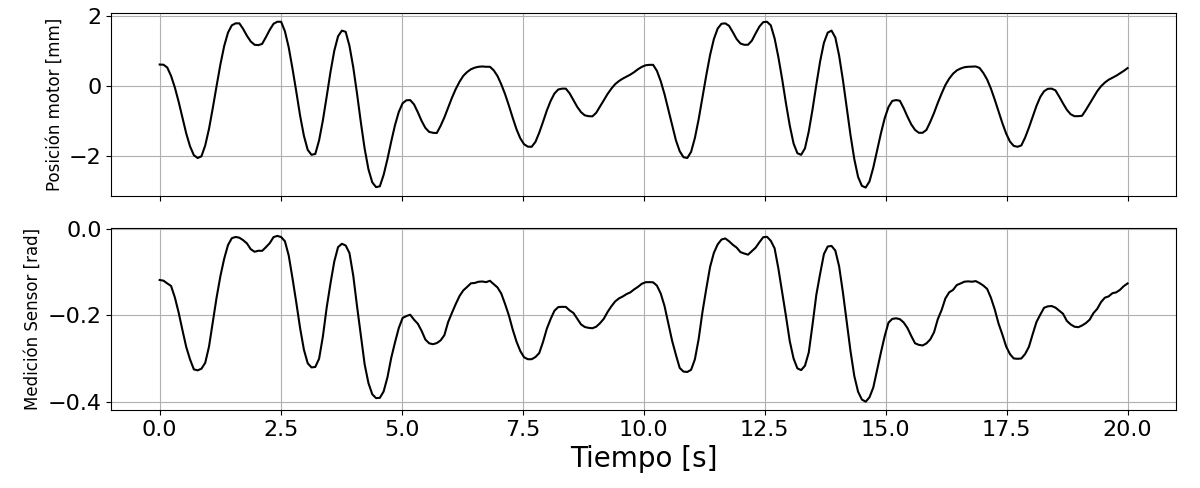
\includegraphics[width=0.87\linewidth]{Figures/08_09_2025/Comparación_alineadas_con_correlación}
	\caption{Arriba posición real del motor lineal, abajo altura de la superficie libre medida por el sensor capacitivo fijo. Notar las claras similitudes entre ambas señales. Se alinearon usando la máxima correlación cruzada. }
	\label{fig:comparacionalineadasconcorrelacion}
\end{figure}

Además si graficamos una contra la otra vemos que la relación es efectivamente lineal, y que no se observa histéresis en los distintos ciclos. 

\begin{figure}[th!]
	\centering
	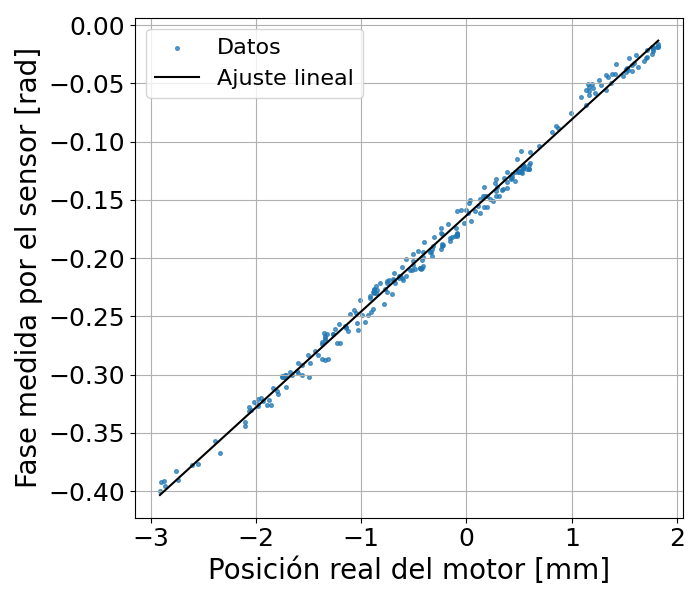
\includegraphics[width=0.543125567\linewidth]{Figures/08_09_2025/Calibración}
	\caption{Gráfico de la posición real del motor vs la señal del sensor. Se puede notar una clara tendencia lineal, con lo cual se muestra también su ajuste por una recta de la forma $f(x) = ax+b$. Parámetros en el texto. }
	\label{fig:calibracion}
\end{figure} 

Los factores de dicho ajuste ($f(x)=ax+b$) fueron: $a=(0.08234\pm0.00036)$ rad/mm, $b=(-0.16340\pm0.00043)$ rad y $R^2=0.995176$. % 5  

Después podemos usar esos factores de calibración para calibrar la señal y estudiar las diferencias entre ambas (en mm). Podemos ver que son del orden de $\pm0.15$ mm como mucho. Podemos ver además que siguen la forma de la señal, o sea, siempre tienen el mismo signo según si la señal sube o baja, lo que sería congruente con que se deban al menisco por capilaridad (Buscar fenómenos de ``Coating" para comparar el orden de ese menisco).  

\begin{figure}[th!]
	\centering
	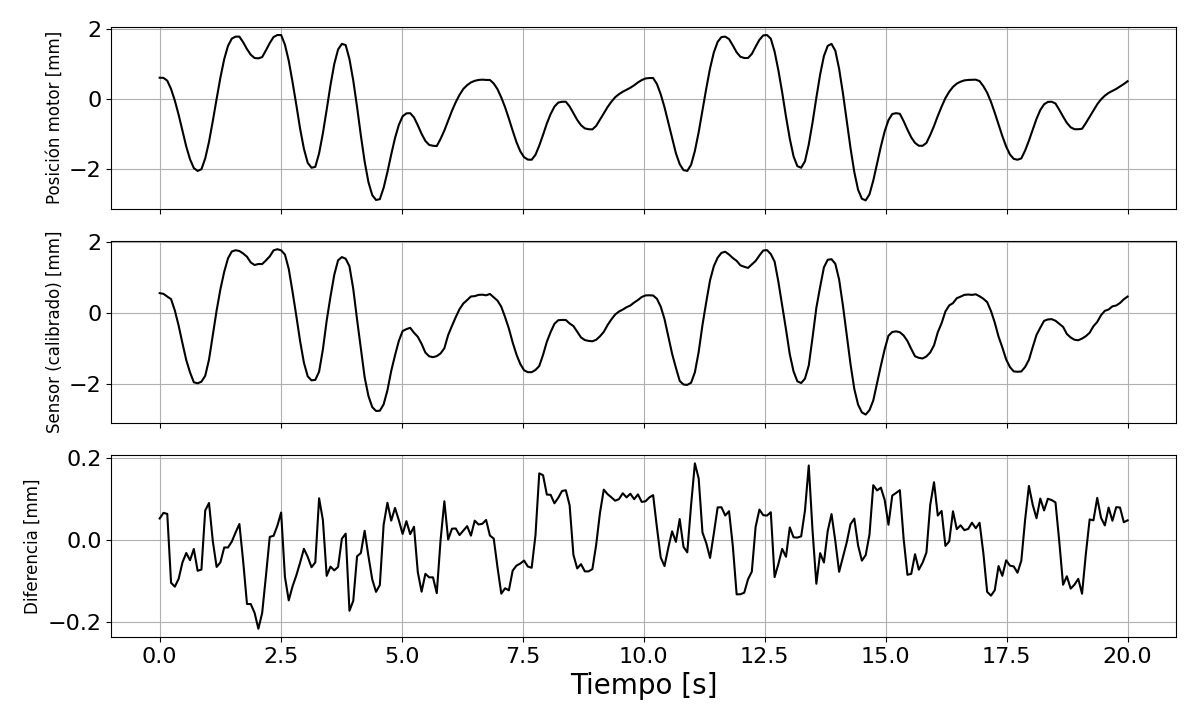
\includegraphics[width=0.87\linewidth]{Figures/08_09_2025/Calibración_diferencias}
	\caption{Mismo que la Figura \ref{fig:comparacionalineadasconcorrelacion} pero habiendo aplicado la función de calibración obtenida a los datos del sensor. Se agregó al final la diferencia entre ambas señales. } % a 
	\label{fig:calibraciondiferencias}
\end{figure}

Por último podemos ver en el histograma de las diferencias que pareciera ser binomial con picos en esos valores de $\pm0.15$ mm y en el espectro un pico importante en frecuencias menores a 1 Hz, que era del orden de las oscilaciones. Ambas cosas parecieran apuntar a que son efectivamente por el menisco y sus inversiones durante la dinámica de la calibración. 

\begin{figure}[th!]
	\centering
	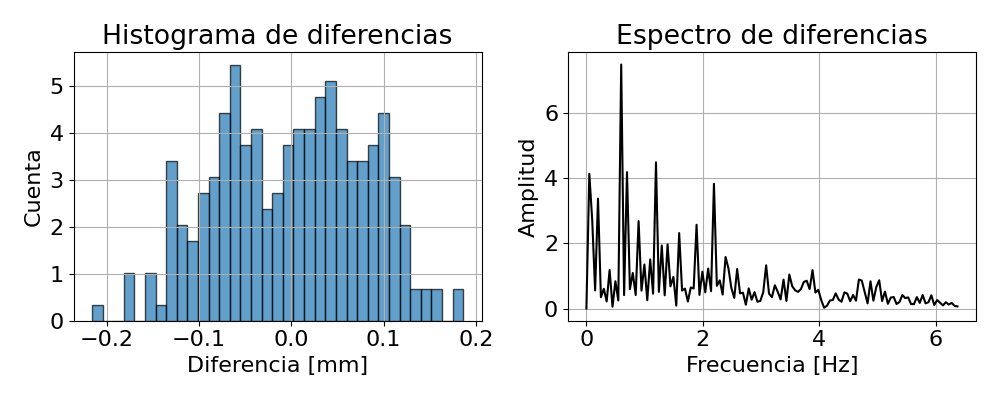
\includegraphics[width=0.87\linewidth]{Figures/08_09_2025/Propiedades_diferencias}
	\caption{Histograma y espectro de las diferencias de la Figura \ref{fig:calibraciondiferencias}.}
	\label{fig:propiedadesdiferencias}
\end{figure}


\clearpage 
\section{Otras Figuras hechas para la charla que vale la pena rescatar. } % 

Por último dejo acá para futuras referencias algunas imágenes que preparé para la charla de la RAFA que me parece quedaron bien y podrían reutilizarse en un futuro.   

\begin{figure}[th!]
	\centering
	\includegraphics[width=0.7\linewidth]{"Figures/08_09_2025/circuito_completo v3"}
	\caption{Esquema del circuito RLC Serie utilizado para medir la capacitancia del sensor.}
	\label{fig:circuitocompleto-v3}
\end{figure}


\begin{figure}[!ht]
	\begin{minipage}[c]{0.5\textwidth}
			\begin{subfigure}{\textwidth}
					\centering
					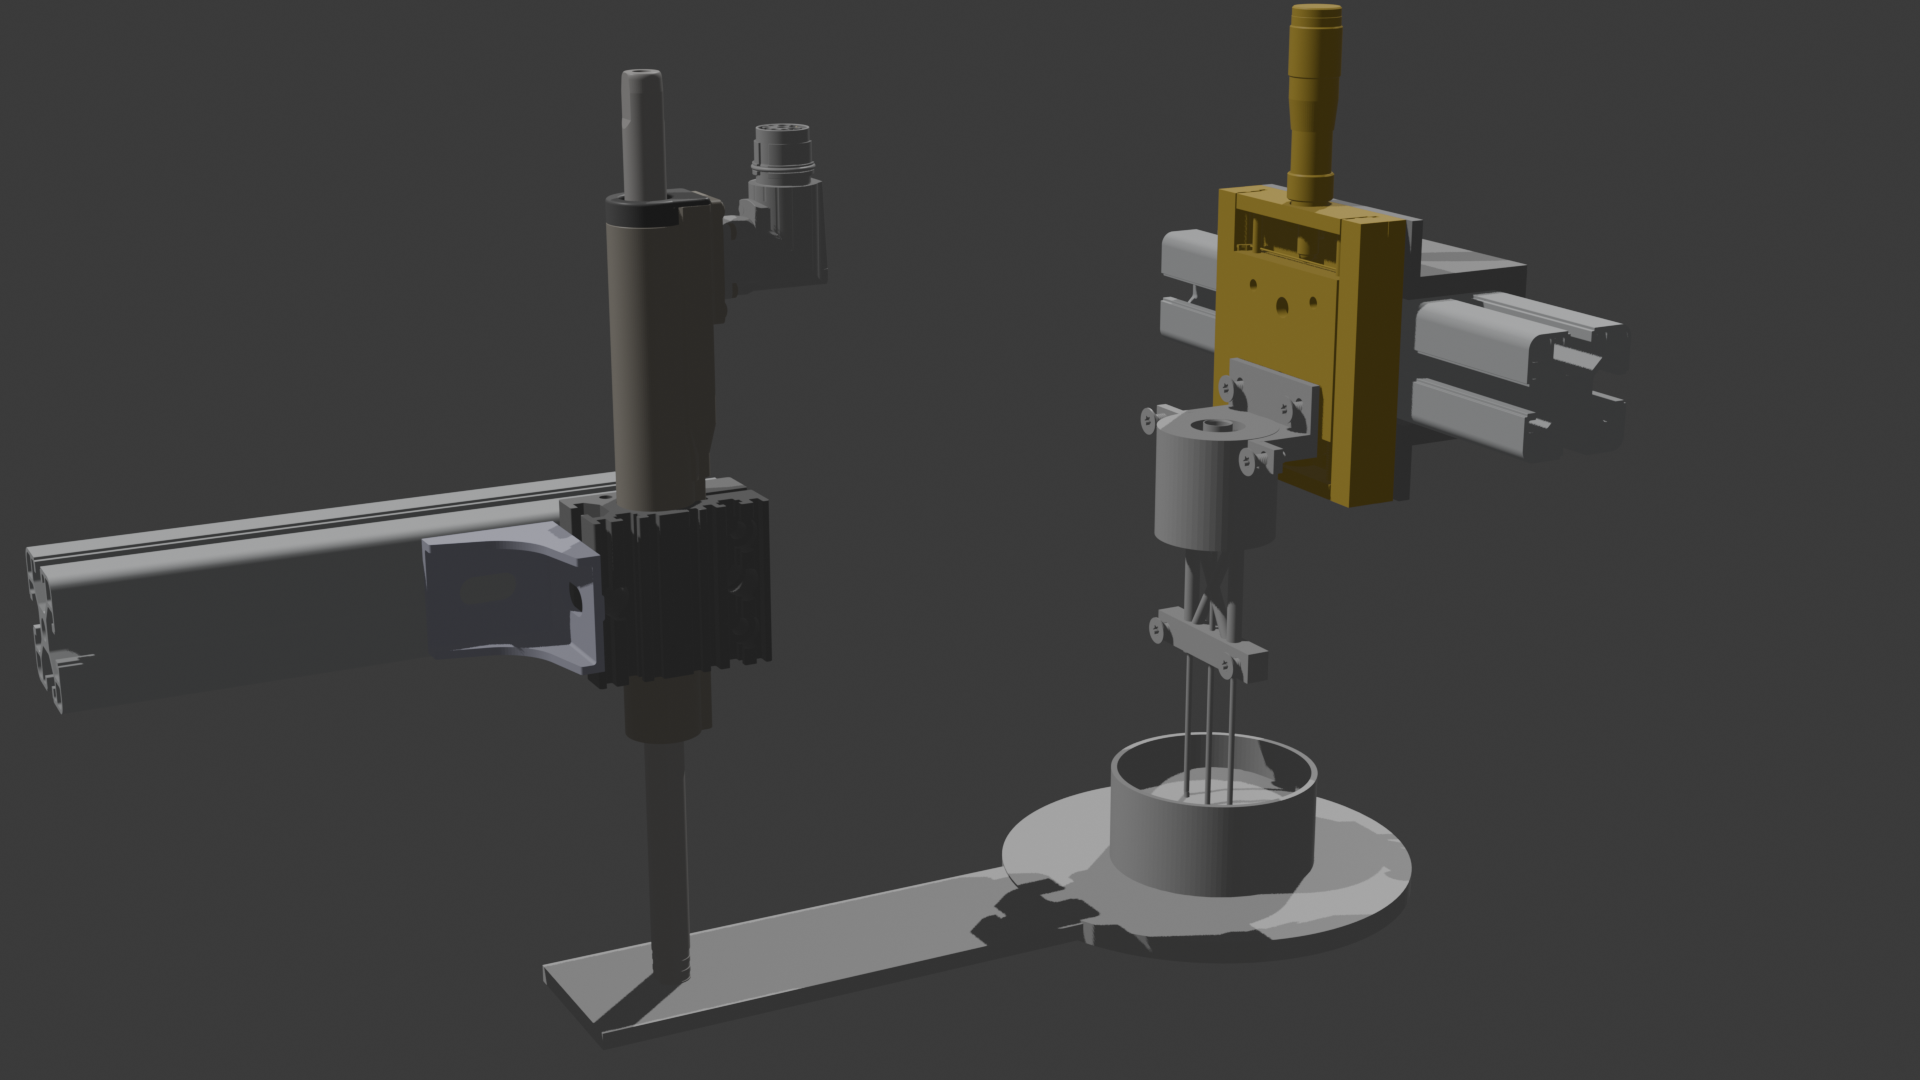
\includegraphics[width=0.8\textwidth]{Figures/08_09_2025/Montaje_calibracion.png}
					\captionsetup{width=0.8\textwidth}
					\subcaption{Calibración Sensor.}
					\label{fig:}
				\end{subfigure}
		\end{minipage}\begin{minipage}[c]{0.49\textwidth}
			\begin{subfigure}{\textwidth}
					\centering
					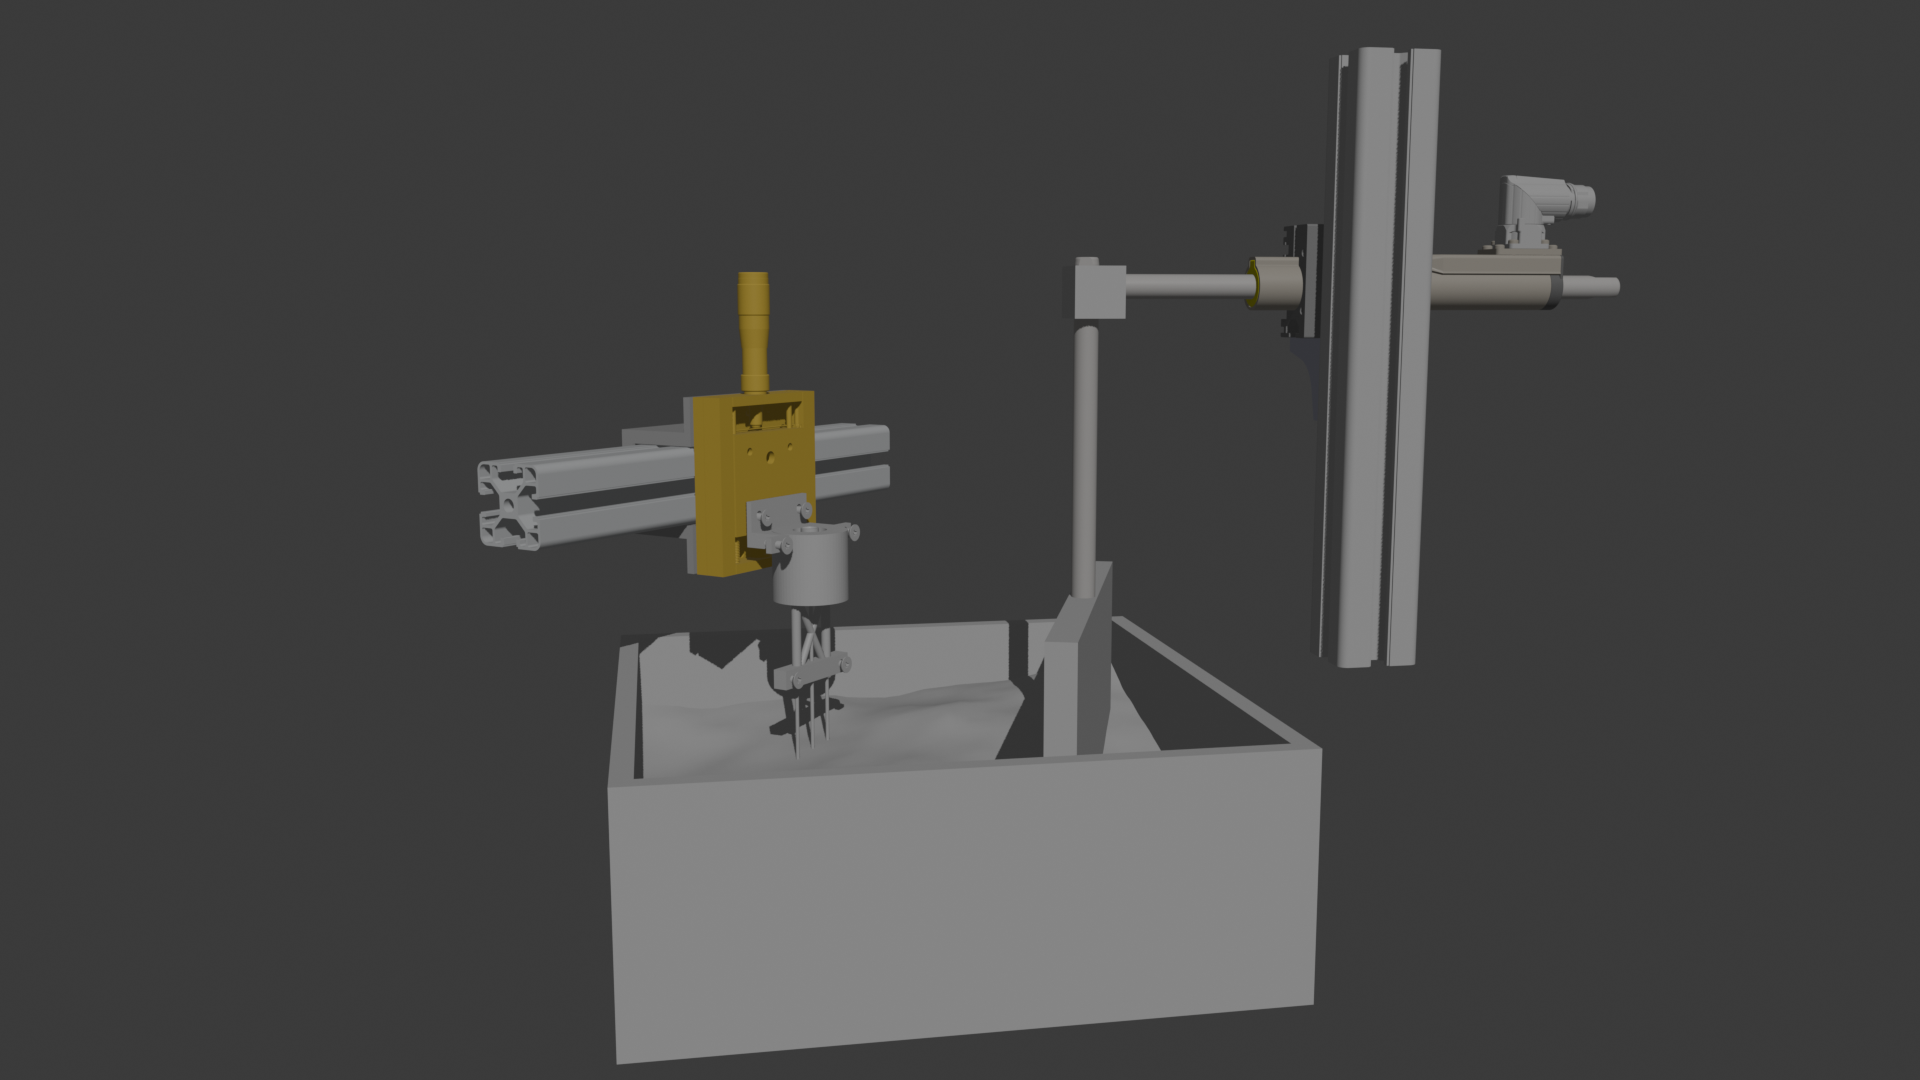
\includegraphics[width=0.8\textwidth]{Figures/08_09_2025/Montaje_wave_turbulence .png}
					\captionsetup{width=0.8\textwidth}
					\subcaption{Turbulencia de Ondas.}
					\label{fig:}
				\end{subfigure}
		\end{minipage}
	\caption{Renders de los montajes relevantes para la calibración del sensor y su utilización en la experiencia típica de turbulencia de ondas.}
	\label{fig:renders_montaje_RAFA} 
\end{figure} 



